\chapter{Event Simulation and Object Reconstruction}\label{chapter:data-mc}
After triggered events from the CMS experiment have been read out, the reconstruction of the reconstruction of the particles produced by the proton-proton collision is performed.
Monte Carlo (MC) simulations, which provide a detailed, precise and realistic description of the expected SM and potential BSM processes, form an essential component of performing any physics analysis.
MC is used for optimising signal extraction strategies and for 

 
The event simulation and objection reconstruction algorithms which are relevant to the single top physics search presented in this thesis are discussed in this chapter.

\section{Event Simulation}\label{sec:sim}
As MC simulation is meant to provide a realistic description of physics processes, both accurate modelling of these processes and a detailed understanding of how physical processes interact with the CMS detector are required to produce events in the same format as raw proton-proton collision data prior to undergoing the same reconstruction process.


%In hadron collisions,
%
%As model hadron collision we need
%As a hadron contains not jist sea of gluons and quarks from the continuous gluon splitting inside it in addition to its constituent valence quarks, 
%
%For the accurate modelling of hadron collisions, knowledge of the internal structure of each hadron 
%
%The inability to directly measure 
%Another difficulty arises from colour confinement preventing 
% the accurate modelling 
%
%The 
%continual gluon splitting inside a hadron results in it  
%As colour confinement results in a hadron containing not only its constituent valence quarks but also a sea of gluons and quarks from the continuous gluon splitting inside
%
%Consequently, as a hadron consists of not only its constituent valence quarks but also a  it~\cite{coughlan2006ideas,evenish2004deep}.
%The first evidence of the 
%The probing of the proton through Deep Inelastic Scattering (DIS) is used to experimentally determine how the number 
%
%
%
%each constituent valence quark within a hadron does not possess an equal fraction of the hadron's momentum due to the 
%Given that 
%As colour confinement prevents a hadron's constituent elements being ..., their internal structure is probed  using 
%\editComment{PDFs and DIS to be added}
%
%PDFs are an essential component of modelling hadron collisions
%
%~\cite{evenish2004deep} - DIS

The simulation of events is a four stage process: generation, simulation, digitisation and reconstruction.

The initial generation stage involves the use \emph{event generators} to simulate the proton-proton interactions and the resultant physics processes~\cite{Buckley:2011ms,Hoche:2014rga}.
The first stage of this is the modelling of the colliding protons and the hard scattering of their constituent partons, which involves the use Parton Distribution Functions (PDFs) to assign fractions of the proton's momentum to the partons and perturbation theory to compute the Matrix Elements (ME) of the Feynman diagrams for the QCD and electroweak processes involved.
The second stage models resultant Parton Showers (PS) through an iterative process until the infrared cutoff scale for the shower is reached and perturbation theory no longer applies.
The remaining particles undergo hadronisation using non-perturbative modelling process.
The various event generators used in the production of MC samples used in this thesis are discussed in Section~\ref{subsec:eventGenerators}.

Following the generation stage, the simulation and digitisation stages involves passing the GEN output through a complete simulation of the CMS detector that has been with the GEANT4 program~\cite{geant4,Lefebure:1999wja}.
This process models particle interactions and decays and the propagation of particles through the detector, the effects of solenoidal field and detector material.
The DIGI stage uses the SIM output to produce the detector's electronics response, which then undergoes the same reconstruction process that data does, as described in Section~\ref{sec:reco}.

The inelastic proton-proton interactions, typically called pileup (\PU), which occur both within and adjacent to the event's bunch crossing, referred to as \emph{in-time} and \emph{out-of-time} \PU  respectively, also require modelling in simulation.
Simulated \PU however, does not adequately describe observed \PU in data.
Therefore, the reweighting of the simulated samples is required and is discussed in Section~\ref{subsec:puSF}.

\subsection{Event Generators}\label{subsec:eventGenerators}
A number of event generators are used by CMS to produce the MC simulation samples used to describe the expected processes produced.
While there are several general-purpose event generators that can describe an event from the initial hadron collision to final state particles, 

they are typically used in conjunction with generators that specialise in a specific physics aspect (\ie ME calculations or PS simulation) or process (\eg tau decays) in order to provide a complete event.

Perturbative calculations of the MEs of the QCD and electroweak processes are done, where possible, to Next-To-Leading Order (NLO) in order to both enable precision measurements to be made and to accurately model processes that include multiple high energy jets.

The MC event generators used to model the background and signal processes for the analysis presented in this thesis are as follows::

\begin{itemize}
%\item \textbf{Madgraph} - Madgraph~\cite{Alwall:2011uj} is a package which performs tree-level perturbativecalculations to produce matrix elements at Leading Order (LO) for processes %such as decays and 2 $\rightarrow$ n scatterings through evaluating the ME for a given phase space point for all the Feynman diagrams produced.
\item \textbf{Madgraph} - Madgraph~\cite{Alwall:2011uj} is a package that performs tree-level perturbative calculations to produce matrix elements at Leading Order (LO) for processes through evaluating the ME for a given phase space point for all the Feynman diagrams produced.
\item \textbf{aMC@NLO} - aMC@NLO~\cite{Alwall:2014hca} is a package that considers tree-level and one-loop Feynman diagrams to produce matrix elements at NLO.
Considering the constructive and destructive interferences which result from considering both the leading and higher order cross section terms results in positively and negatively weighted events.
These negatively weighted events are not simply discarded as they are required to correctly simulate the NLO cross section by applying a scale factor, $SF^{NLO}$, which considers the ratio of the total number of events to the effective number of events (\ie the difference in positively and negatively weighted events) in the sample and the sign of an individual event's weighting:
\begin{equation}
SF^{NLO} = \frac{N^{postive events} + N^{negative events}}{N^{postive events} - N^{negative events}} \times \frac{|event weight|}{event weight} \;
\end{equation}

\item \textbf{POWHEG} - The Positive Weight Hardest Emission Generator (POWHEG)~\cite{Alioli:2010xd} is a framework that interfaces NLO ME calculations with PS generators.
As its name suggests, POWHEG produces the hardest emission first through using the exact NLO ME and produces only positively weighted events.
The latter is achieved by interfacing to a PS generator which order emissions by \pT or allows for the use of a $p_{T}$-veto to reject subsequent emissions, avoiding double counting such emissions and the need for negative weights.
\item \textbf{PYTHIA} - PYTHIA~\cite{Sjostrand:2014zea} is a general-purpose generator which capable of taking the output of a ME event generator and perform the parton showering and hadronisation to produce the full event. For all of the MC samples considered in Section~\ref{sec:samples} for the analysis presented, PYTHIA 8 is used to develop the samples from their ME event generator output into a full event.
\end{itemize}

\section{Object Reconstruction}\label{sec:reco}
Using the output of all the CMS sub-detectors, a full reconstruction of the triggered physics event is undertaken.
This process involves the \emph{Particle Flow} (PF) algorithm, which combines complementary information from each of the CMS sub-detectors, known as \emph{elements}, to provide an optimal reconstruction and identification of all stable particles present in the event~\cite{CMS:2009nxa,CMS:2010eua,CMS-PRF-14-001}.
Using these reconstructed particles, additional objects such as b-jets and missing transverse energy can also be identified.

\subsection{Charged Particle Tracks}\label{subsec:tracks}
As the charged particles produced in proton-proton collisions traverse the silicon tracker, they interact with it and leave energy deposits on the individual layers, known as \emph{hits}.
These hits are used to reconstruct the particles' trajectories using the Combinatorial Track Finder (CTF) algorithm, which is based on combinatorial Kalman Filtering~\cite{Chatrchyan:2014fea,Fruhwirth:1987fm}.

The CTF algorithm is iterative and consists of the following steps:
\begin{itemize}
\item \textbf{Seed generation:} Initial track candidates are formed from two or three hits in the inner part of the track in order to provide a first estimate of the tracks' helix parameters.
\item \textbf{Track Finding:} A combinatorial Kalman Filter then builds a candidate by adding hits from successive layers that are compatible with the extrapolated trajectory. The candidate is updated with the addition of each subsequent hit, taking into account the hit's position, uncertainty and material traversed.
\item \textbf{Track Fitting:} The initial estimate of a track's parameters is improved using two additional passes of the KF.
The first pass minimises the bias from the seed generation step by working from the innermost layer outwards.
The second minimises the bias from the track finding step by working from the outermost layer inwards.
By performing these two passes any bias in the identification of incorrectly associated hits is minimised.
\item \textbf{Track Selection:} Quantities, such as $\chi^{2}$, the number of layers with hits and compatibility, are used to identify and reject tracks that have been incorrectly reconstructed.
\end{itemize}

Up to six iterations of the CTF are performed, with selected tracks' hits removed from consideration in subsequent iterations, in order to ensure that 

The initial four iterations use seeds exclusively from the pixel tracker and the last two iterations use seeds from the strip tracker.
By using seeds from the outer part of the tracking detector, to enable a high track reconstruction efficiency for those originating outside the pixel detector or those that did not leave any hits in the pixel tracker.

\subsection{Primary Vertices}\label{subsec:vertices}
The reconstructed tracks described above are used to reconstruct the positions where the proton-proton collisions occurred, known as \emph{primary vertices}~\cite{Chatrchyan:2014fea,Speer:2006mh}.
Tracks are considered for primary vertex reconstruction if they are consistent with originating promptly from the interaction region, namely having a small $d_{0}$, a minimum number of hits in the pixel and strip trackers and a low $\frac{\chi^{2}}{ndf}$.
Tracks meeting those requirements are then clustered along the z-axis at their point of closest approach to the beamspot using a deterministic annealing algorithm~\cite{Kenneth:1998i}.
An adaptive vertex fitter is used to produce a 3D fit of the vertex track candidates and determine their uncertainties and variables such as the number of degrees of freedom to discriminate against fake vertices~\cite{Fruhwirth:2007hz}.
Out of the resulting track candidates, the one with the greatest scalar transverse momentum is considered as the \emph{primary vertex}, with the rest being assumed to represent \PU vertices.
Displaced vertices, such as those from the decay of heavy hadrons, are identified later in the reconstruction process.

\subsection{Calorimeter Energy Clusters}\label{subsec:clustering}
The energy deposited by particles in the calorimeters is independently clustered in each sub-detector, except for the HF where each large cell gives rise at most to just one cluster, to determine the energy and direction of the particles~\cite{CMS:2009nxa}.

The clustering algorithm consists of three steps:
\begin{itemize}
\item \textbf{Cluster seeding:} Local cells with energies above a certain threshold are identified and considered as seeds.
\item \textbf{Clustering:} Adjacent seed cells are summed together to form seed clusters.
\item \textbf{Energy threshold:} A cluster is retained for further use if its energy is greater than two $\sigma$ above the expected electronics noise in that part of the calorimeter (80\MeV in the EB, 300\MeV in the EE, and 800\MeV in the HCAL).
\end{itemize}

\subsection{Particle Flow Algorithm}\label{subsec:PF}
Through combining clusters in the calorimeters and charged particle tracks from the tracker and muon systems, the Particle Flow algorithm is able to use all the available information from an event to reconstruct and identify all the stable particles that it contains with far superior results than if each sub-detector were used individually~\cite{CMS-PRF-14-001}.

The first stage of the algorithm involves associating or \emph{linking} charged particle tracks with clusters in the calorimeters and between clusters in the different calorimeters.
Following this, the linked elements are used by the PF algorithm to sequentially reconstruct and identify different PF particles types.
As PF particles are identified, their associated tracks and clusters are removed from further consideration.

Charged particle tracks are linked to clusters by extrapolating a track's last measured hit in the tracker to the calorimeter systems.
If a track's expected position in the calorimeters are within a clusters' boundaries, these elements are linked together.
Similarly, tangents to the inner tracker tracks are extrapolated to the ECAL in order to identify  and link tracks to Bremsstrahlung photons.
Calorimeter cluster links are formed if a cluster from the higher granularity detector (ECAL/ES) lies within the acceptance boundaries of the lower granularity detector considered (HCAl/ECAL).

The different particle types are then reconstructed in the following order: 
\begin{itemize}
\item muons (see Section~\ref{subsec:objReco-muons}).
\item electrons, associated Bremsstrahlung photons and isolated photons (see Section~\ref{subsec:objReco-electrons}).
\item HCAL clusters which are compatible with the remaining ECAL clusters and charged particle tracks are classified as charged hadrons.
\item any remaining ECAL and HCAL clusters with no associated charged particle tracks are classified as photons and neutral hadrons, respectively.
\end{itemize}

After all these particle types are reconstructed, a post-processing stage is undertaken to mitigate against the small probability mis-identifying or reconstructing particles, usually high momentum muons. 
This avoids the appearance of an apparently large amount of missing transverse energy being present in an event.

\subsection{Electrons}\label{subsec:objReco-electrons}
Electrons lose, on average, between 33\% (minimal intervening material) and 86\% (maximum intervening material) of their energy before reaching the ECAL through the production of Bremsstrahlung photons in the tracker layers~\cite{Khachatryan:2015hwa}, which often undergo electron pair production, potentially producing further Bremsstrahlung photons.	
It is essential that this radiated energy is collected in order to correctly determine the electron's initial energy.

As the magnetic field bends electrons trajectories in the $\phi$ direction, their is energy across $\phi$, the ECAL crystals are clustered into strips in $\phi$ known as \emph{superclusters} (SCs).
Two clustering algorithms are used to form SCs of $5 \times 1$ and $5 \times 5$ arrays of ECAL crystals in the EB and EE respectively due to their different geometrical arrangements~\cite{Khachatryan:2015hwa}.
In the EB, the so-called \emph{hybrid} algorithm builds SCs.
The algorithm initially identifies a seed crystal which contains at least $E_{T} > 1\GeV$ and contains the largest energy deposit for a given region.
Arrays of $5 \times 1$ crystals in $\eta \times \phi$, which contain at least $E_{T} > 0.1\GeV$ and are within $\Delta \phi < 0.3$ of the seed crystal, are clustered together to form the SC.
The so-called \emph{multi $5 \times 5$} algorithm builds SCs in a similar manner in the EE.
Seed crystals are required to contain at least $0.18\GeV$, and the arrays of $5 \times 5$ crystals added to the SC if the array has $E_{T} > 1\GeV$ and is within $\Delta \phi < 0.3$ and $\Delta \eta < 0.07$ of the seed crystal.

The presence of Bremsstrahlung photons also necessitates the use of a Gaussian Sum Filter (GSF)~\cite{Adam:2003eca} to fit electron tracks instead of a Kalman Filter as the process is non-Gaussian and Kalman Filters assume only Gaussian noise contributions.
The computationally heavy nature of the GSF algorithm, however, limits its use to refitting \KF track seeds and for the final fitting of the electron track parameters.

%%% Track seeding
Electron track seeds, formed of the initial two or three hits in the tracker from which tracks are built,  are constructed using two complimentary algorithms~\cite{Khachatryan:2015hwa}:
\begin{itemize}
\item \textbf{ECAL-based approach} An electron's SC's energy and position is used to extrapolate the expected electron trajectory towards the primary vertex to determine where associated tracker hits would be expected for both electrons and positrons.
Reconstructing electrons in jets however, suffers from large inefficiencies. 
This is due to the potential to incorrectly associate hits from other charged particles with the electron track and impact of jet energy deposits overlapping with the electron SC on the electron's assumed energy and position.
Low \pT electrons are also poorly reconstructed as the increased bending of their trajectories results in the spread energy not being fully contained within a single SC.

\item \textbf{Tracker-based approach} This approach is designed to compliment the ECAL-based approach by reconstructing non-isolated and low \pT electrons efficiently.
A \KF (KF) is initially used for track finding as it is able to accurately reconstruct electrons that emit only a small amount of Bremsstrahlung in the tracker, with the KF track being matched to the closest ECAL SC.
Tracks that are indicative of the emission of a significant amount of Bremsstrahlung are refitted with a GSF.
Track parameters from both filters, such as the quality ($\chi^{2}$) and how well matched the track is to the ECAL SC, are used by a Multivariate Analysis (MVA) technique to determine whether or not the tracker seed can be used as an electron seed.
\end{itemize}

The seeds collections produced by both algorithms are merged into a single set of seeds.
From this combined set of seeds, electron tracks are iteratively built using as combinatorial \KF in which a series of cuts are applied in order to accommodate trajectory changes due to Bremsstrahlung and to maintain a high reconstruction efficiency.
These electron tracks undergo a final fitting by the the GSF to precisely determine the electron track parameters.

\subsection{Muons}\label{subsec:objReco-muons}
Muon tracks are independently reconstructed in both the inner tracker, as described in Section~\ref{subsec:tracks}, and the muon chambers.
Track reconstruction in the muon chambers is undertaken using a Kalman Filter to build tracks from the innermost track segments made up of clustered DT and CSC hits outwards using DT, CSC and RPC hits.

These two types of muon tracks are reconstructed using two methods~\cite{Chatrchyan:2012xi}:
\begin{itemize}
\item \textbf{Global Muons} are reconstructed using an ``\emph{outside-in}'' approach, where tracks in the muon chambers are extrapolated inwards towards the inner tracker where candidate tracks are then searched for.
If a corresponding track is found, the hits from the best candidate in the inner tracker and the muon system are fitted using a Kalman Filter to form a Global Muon.
\item \textbf{Tracker Muons} are conversely reconstructed with an ``\emph{inside-out}'' approach, where inner tracker tracks with $\pT > 0.5\GeV$ and $|p| > 2.5\GeV$ are extrapolated out to the muon system using a Kalman Filter that takes into account energy losses and multiple scattering.
If at least one one muon segment in the muon chambers is consistent with the extrapolated muon track, the track is classified as a Tracker Muon.
\end{itemize}

Given the high track reconstruction efficiencies of both the inner tracker and the muon chambers, approximately $99\%$ of muons produced from the proton-proton collisions (prompt muons) are reconstructed as either a global or tracker muon, if not both.
Global and tracker muons that share the same inner tracker track are merged into a single candidate muon to be considered by the PF algorithm.

\subsection{Jets}\label{subsec:objReco-jets}
Due to colour confinement, quarks and gluons produced in a proton-proton hard interaction rapidly hadronise, producing a collimated shower of hadrons that are clustered and reconstructed as \emph{jets}~\cite{Salam:2009jx}.
Any jet reconstruction algorithm is required to be both \emph{infrared safe} and \emph{collinear safe}, \ie so that the emission of soft gluons and the collinear splitting of gluons, respectively, do not change the jets that are actually constructed.

The main two types of jet algorithms are iterative cone and sequential recombination algorithms~\cite{Salam:2009jx}, and while both varieties are supported by CMS, the latter are typically used in the majority of analyses.

The general form of a sequential recombination algorithm is as follows:
\begin{itemize}
\item The distance, $d_{ij}$, for every pair of particles and the distance between each particle and the beamline, $d_{iB}$, is calculated.
\item If the minimum value of $d_{ij}$ is less than $d_{iB}$, the pair of particles are recombined into a single particle, and the process starts over.
\item If the minimum value of $d_{iB}$ is less than $d_{ij}$, the particle is classified as a jet and removed from the list of particles under consideration, and process begins again.
\end{itemize}

The process continues until no particles remain on the list.

These distance variables are defined as:

\begin{equation}
d_{ij} = min(p^{2k}_{Ti},p^{2k}_{Tj}) \frac{\Delta R^{2}_{ij}}{R^{2}} \;
\label{eq:jetAlgo1}
\end{equation}

\begin{equation}
d_{iB} = \frac{1}{p^{2k}_{Ti}} \;
\label{eq:jetAlgo2}
\end{equation}

where $\Delta R^{2}_{ij} = (y_{i} - y_{j})^{2} + (\phi_{i} - \phi_{j})^{2}$; k = ${-1, 0, 1}$ and R is the jet size parameter, which is typically set to 0.4 in CMS analyses to provide consistency with ATLAS and as it has been found to contain hadronic showers without being sensitive to \PU.
The \emph{anti-\kt} algorithm~\cite{Cacciari:2008gp}, where k = -1, which produces cone-shaped jets, is commonly used in CMS.
The other values of k, where k = $0,1$, correspond to the Cambridge/Aachen and \kt algorithms respectively.

PF jets are produced using the \emph{anti-\kt} algorithm with R = 0.4 in conjunction with PF particles based on all the sub-detectors.
Making use of PF jets allows a more accurate reconstruction to be undertaken than if only energy clusters from the calorimeters are used, given that jets are typically composed of 65\% charged hadrons, 25\% photons and 10\% neutral hadrons, due to the precise charged hadron measurements from the tracker and ECAL, which are able to constrain the small neutral hadron contribution that relies on the relatively poor resolution of the HCAL.

\subsubsection{Jet Energy Corrections}\label{subsubsec:JECs}
\emph{Jet Energy Corrections} (JECs) are used to take into account the effects of \PU and the non-uniform response in \pT and $\eta$ of the detector and any residual differences between simulation and data.
Each of these effects is considered as a separate correction level; they are applied sequentially through the use of a scale factor applied to a jet's four-momentum in the following order:

\begin{itemize}
\item \textbf{L1 Pileup.} Removes additional energy originating from \PU interactions from the jet energy and is applied to both data and simulated events. 
\item \textbf{L2 Relative and L3 Absolute} Applied to data and simulation to account for the non-uniform detector response in $\eta$ and \pT, respectively. The scale factor is derived by comparing generator level and reconstructed jets in the simulation.
\item \textbf{L2L3 Residual} Applied to data only to account for any remaining small differences in the jet response between data and simulation, such as the absolute Jet Energy Scale (JES) following application of the previous corrections..
\end{itemize}

The uncertainties associated with these JECS are treated as systematic uncertainties, which are discussed in Chapter~\ref{sec:systematics}.
Further details regarding the JECs can be found in~\cite{Khachatryan:2016kdb}.

\subsection{b-tagging}\label{subsec:objReco-bJets}
Correctly determining whether or not a jet was the product of a b-quark hadronising is important for a variety of analyses, allowing them to better separate signal processes from topologically-similar background processes.
b-jet identification is particularly pertinent for top physics searches due to the fact that the dominant decay mode for a top quark is to a W boson and a b-quark~\cite{Tanabashi:2018oca}.

This process is known as \emph{b-tagging} and exploits the fact that because b-hadrons have a relatively long lifetime of approximately 1.5 ps~\cite{Beringer:1900zz}, they can travel a measurable distance away from the primary vertex before decaying. 
The resulting secondary vertices are exploited in b-tagging, which is performed in CMS by a number of algorithms supported by the CMS B-Tag and Vertexing (BTV) Physics Object Group.
The analysis presented uses the \emph{Combined Secondary Vertex} version 2 (CSVv2) algorithm~\cite{Sirunyan:2017ezt}.
The CSVv2 algorithm uses information about displaced track and secondary vertices as input into a multilayer perceptron (a class of neural network) to produce a discriminator value which characterises the likelihood that the likelihood a jet originated from a b-quark.

Three different \emph{working points} (loose, medium and tight) are defined by the BTV POG for b-tagging algorithms, such that the probability for incorrectly tagging light flavoured jets is 10\%, 1\% and 0.1\% respectively.
Figure~\ref{bTagEffVsMisId} illustrates the negative impact that minimising the light jet misidentification probability has on the efficiency at selecting genuine b-jets for the b-tagging algorithms supported within CMS~\cite{Sirunyan:2017ezt}.

\begin{figure}[tbp]
\centering
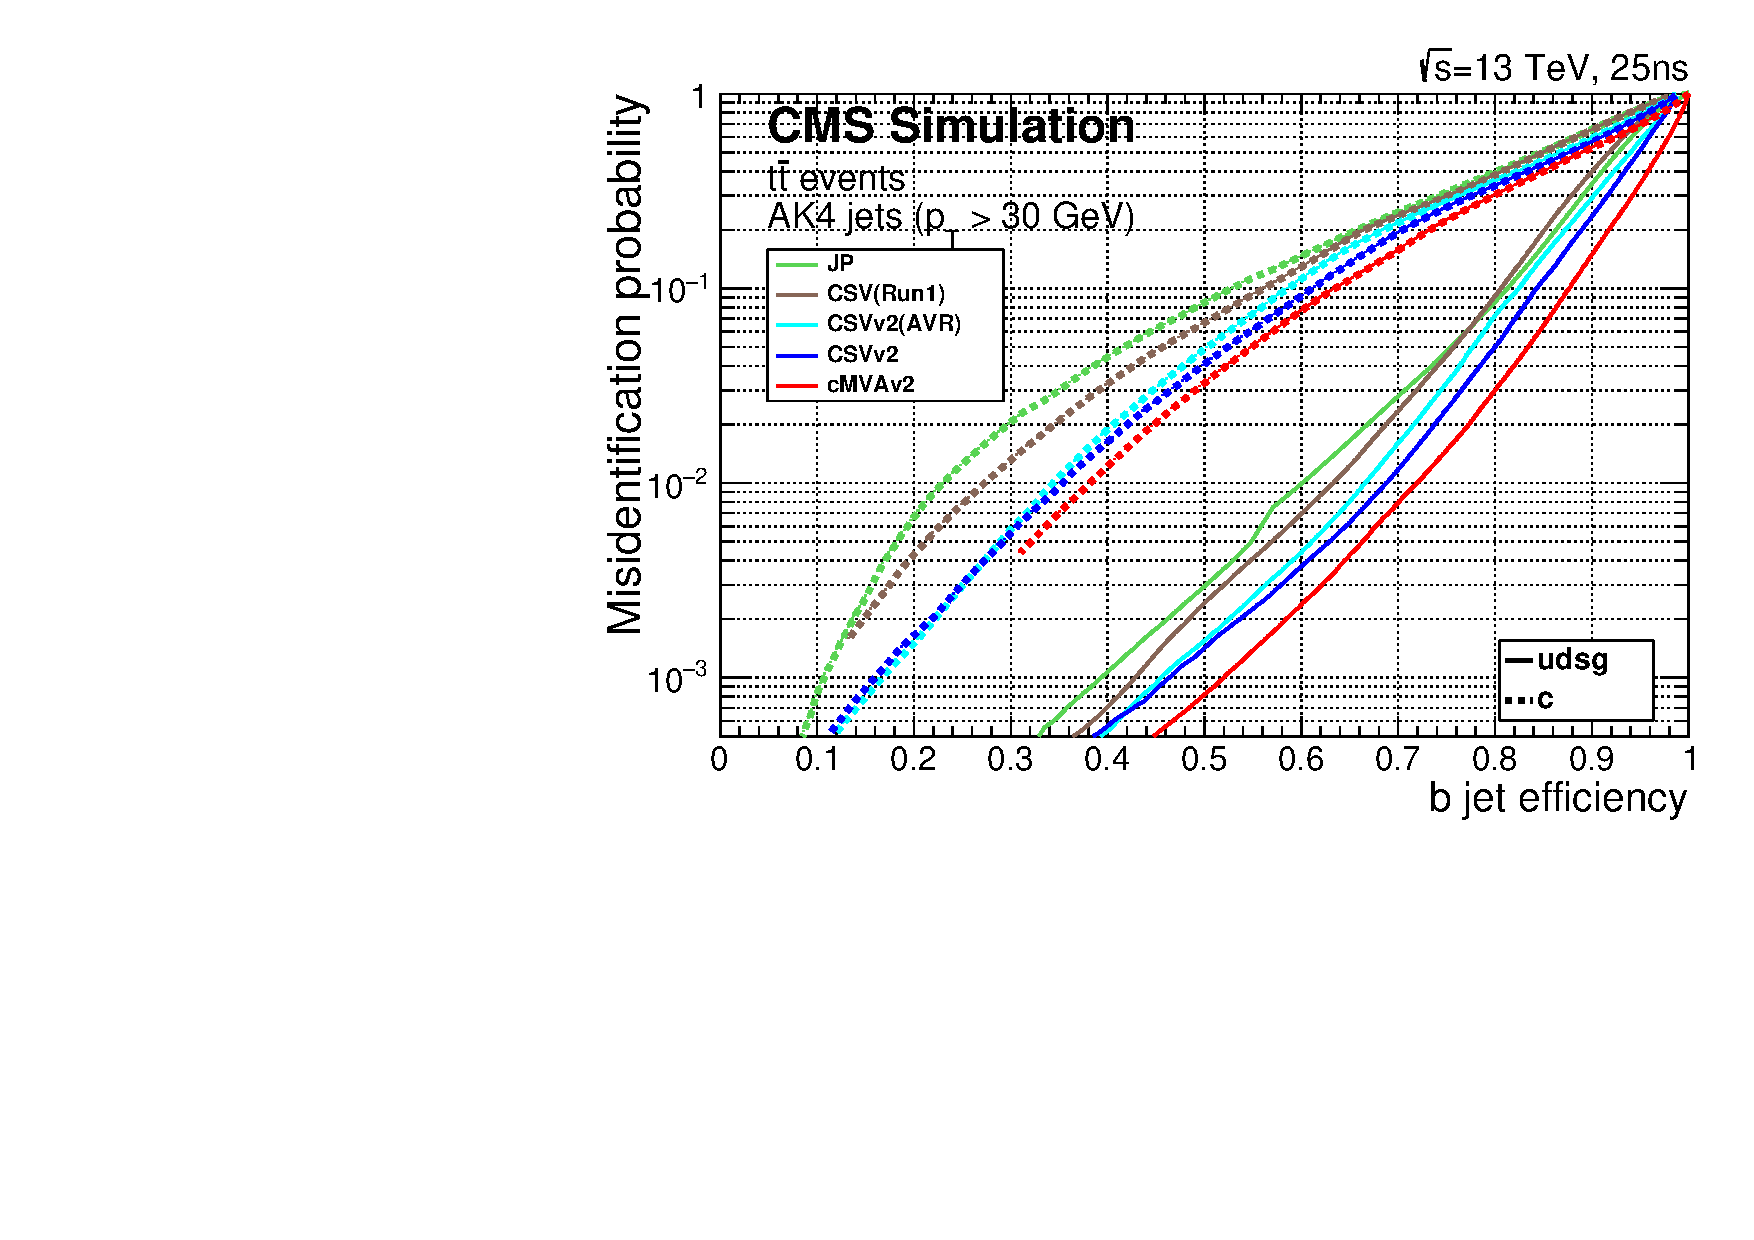
\includegraphics[width=\textwidth]{figs/data-mc/effVsMisTagcsvV2.pdf}
\caption{The light flavoured jets misidentification probability as a function of the efficiency of tagging genuine b-jets for the b-tagging algorithms supported within CMS~\cite{Sirunyan:2017ezt}.}
\label{fig:bTagEffVsMisId}
\end{figure}

The selection efficiencies for b-jets, c-jets and light jets for each of the working points for the CSVv2 algorithm are given in table~\ref{tab:bTagWPs}.

\begin{table}[htbp]
\topcaption {
The CSVv2 algorithm's selection efficiencies and mis-identification rates for each of the three working points for b-($\epsilon_{b}$), c-($\epsilon_{c}$), and light jets ($\epsilon_{udsg}$) with $\pT > 20\GeVc$ in simulated \ttbar events~\cite{Sirunyan:2017ezt}.
}
\label{tab:bTagWPs}
  \centering
% This increases column spacing.
  \addtolength{\tabcolsep}{1ex}
% This right-aligns numbers in column, but centers them under column title.
  \begin{tabular}{ccr@{\hspace{4ex}}r@{\hspace{4ex}}r@{\hspace{4ex}}r@{\hspace{4ex}}}
   \hline

   \hline
   \textbf{CSVv2 WP Name (value)} & \textbf{$\epsilon_{b}$ (\%)} & \textbf{$\epsilon_{c}$ (\%)} & \textbf{$\epsilon_{udsg}$ (\%)}   \\
   \hline
   Loose (0.5426) & 84 &  39 & 8.3 \\
   \hline
   Medium (0.8484) & 66 &  13  & 0.8\\  
   \hline
   Tight (0.9535) & 46 &  2.6 & 0.1 \\  
   \hline
   
 \end{tabular}
 \addtolength{\tabcolsep}{-1ex}
\end{table}

\subsection{Missing Transverse Energy}\label{subsec:objReco-MET}
Particles that only weakly interact with matter, such as neutrinos and some hypothesised BSM particles, escape the detector without being directly observed.
Their presence however, can be inferred by imposing conservation of transverse momentum to any given event.
The missing energy in the plane transverse to the beam line, $\overrightarrow{\MET}$, is defined as the negative vector sum of the transverse momentum in the event:

\begin{equation}
\overrightarrow{\MET} = - \sum \overrightarrow{\pT} \;
\label{eq:MET}
\end{equation}

There are several different algorithms, using differing variables and techniques, that are used in CMS analyses to determine \MET.

PF \MET, produced using PF particles, is used in this analysis because of its high performance~\cite{CMS:2016ljj}. 
It must however, first be corrected before it can be used.
The so-called \emph{Type-I} \MET corrections replace the PF jets used to determine the \MET of an event with the PF jets with the JECs~\cite{Chatrchyan:2011tn}).